% Drawing 43/04-3 -- folder 43, batch 04, archive page 66 (PDF page 67).
% Transcription: au centre, un croquis : deux cercles sécants et un point
% Kind: two intersecting circles and a point. Method 2 (schematic redraw from the facsimile). Status: ok.
% Notes: Two intersecting circles (the lower one larger) and a point, with a short stroke through it (it looks like a phi written in the circles).
% Coordinates: 1 unit = 1 mm = 1/100 of the crop width (bbox in page fractions: [0.3, 0.45, 0.75, 0.6]).
% Redrawn by Claude (claude-opus-5-5), issue #73, 2026-11-07; not checked by a human; not compiled (no TeX in the session).
% Rights: reproduces part of the work -- behind RENDER_TRANSCRIPTS, never published by itself.
\documentclass[tikz,border=3pt]{standalone}
\usepackage{amsmath,amssymb}
\usetikzlibrary{patterns,arrows.meta}
\tikzset{pencil/.style={black!45}, struck/.style={black!35}, mark/.style={circle,draw,inner sep=1.3pt}, pt/.style={circle,fill,inner sep=0.9pt}, opt/.style={circle,draw,fill=white,inner sep=1.1pt}}
\begin{document}
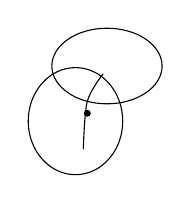
\begin{tikzpicture}[x=1mm,y=1mm,line cap=round,line join=round,font=\scriptsize]
\draw (30,-26.5) ellipse[x radius=6, y radius=6.8];
\draw (34,-19.5) ellipse[x radius=7, y radius=4.8];
\node[pt] at (31.5,-25.5) {};
\draw plot[smooth, tension=0.55] coordinates {(33.5,-20.5) (31.5,-24) (31,-30)};
\end{tikzpicture}
\end{document}
